% do not change these two lines (this is a hard requirement
% there is one exception: you might replace oneside by twoside in case you deliver 
% the printed version in the accordant format
\documentclass[11pt,titlepage,oneside,openany]{article}
\usepackage{times}

\usepackage{url}
\usepackage[hidelinks]{hyperref}
\usepackage{graphicx}
\usepackage{latexsym}
\usepackage{amsmath}
\usepackage{amssymb}

\usepackage{ntheorem}

% \usepackage{paralist}
\usepackage{tabularx}

% this packaes are useful for nice algorithms
\usepackage{algorithm}
\usepackage{algorithmic}

% well, when your work is concerned with definitions, proposition and so on, we suggest this
% feel free to add Corrolary, Theorem or whatever you need
\newtheorem{definition}{Definition}
\newtheorem{proposition}{Proposition}


% its always useful to have some shortcuts (some are specific for algorithms
% if you do not like your formating you can change it here (instead of scanning through the whole text)
\renewcommand{\algorithmiccomment}[1]{\ensuremath{\rhd} \textit{#1}}
\def\MYCALL#1#2{{\small\textsc{#1}}(\textup{#2})}
\def\MYSET#1{\scshape{#1}}
\def\MYAND{\textbf{ and }}
\def\MYOR{\textbf{ or }}
\def\MYNOT{\textbf{ not }}
\def\MYTHROW{\textbf{ throw }}
\def\MYBREAK{\textbf{break }}
\def\MYEXCEPT#1{\scshape{#1}}
\def\MYTO{\textbf{ to }}
\def\MYNIL{\textsc{Nil}}
\def\MYUNKNOWN{ unknown }
% simple stuff (not all of this is used in this examples thesis
\def\INT{{\mathcal I}} % interpretation
\def\ONT{{\mathcal O}} % ontology
\def\SEM{{\mathcal S}} % alignment semantic
\def\ALI{{\mathcal A}} % alignment
\def\USE{{\mathcal U}} % set of unsatisfiable entities
\def\CON{{\mathcal C}} % conflict set
\def\DIA{\Delta} % diagnosis
% mups and mips
\def\MUP{{\mathcal M}} % ontology
\def\MIP{{\mathcal M}} % ontology
% distributed and local entities
\newcommand{\cc}[2]{\mathit{#1}\hspace{-1pt} \# \hspace{-1pt} \mathit{#2}}
\newcommand{\cx}[1]{\mathit{#1}}
% complex stuff
\def\MER#1#2#3#4{#1 \cup_{#3}^{#2} #4} % merged ontology
\def\MUPALL#1#2#3#4#5{\textit{MUPS}_{#1}\left(#2, #3, #4, #5\right)} % the set of all mups for some concept
\def\MIPALL#1#2{\textit{MIPS}_{#1}\left(#2\right)} % the set of all mips





\begin{document}

\pagenumbering{roman}
% lets go for the title page, something like this should be okay
\begin{titlepage}
	\vspace*{2cm}
  \begin{center}
   {\Large IE650 Semantic Web Technologies\\}
   \vspace{2cm} 
   {Project Report\\}
   \vspace{2cm}
   {presented by\\
    Oliver Frendo (1510432) \\
    Sascha Ulbrich (1493181) \\
   }
   \vspace{1cm} 
   {submitted to the\\
    Data and Web Science Group\\
    Prof.\ Dr.\ Paulheim\\
    University of Mannheim\\} \vspace{2cm}
   {December 2016}
  \end{center}
\end{titlepage} 

% no lets make some add some table of contents
\tableofcontents
\newpage

%\listofalgorithms

%\listoffigures

%\listoftables

% evntuelly you might add something like this
% \listtheorems{definition}
% \listtheorems{proposition}

\newpage


% okay, start new numbering ... here is where it really starts
\pagenumbering{arabic}

• 10-12 pages (sharp!) without title and toc pages 
• due Friday, December 2nd, 23:59 
• send by email to Anna Lisa, André and Heiko 
• describe your solution including the steps to get there (chapters already created)

Requirements 
You must use the DWS master thesis layout
Please cite sources properly. Preferred citation style [Author, year]



\section{Application domain and goals}
Which users are targeted? – Which user problems are solved? – Which user information needs are addressed
%@Olli?

\section{Datasets used} 
Which datasets does the application use?
- DBPedia, DBPediaLive, iServe, ... 
How are they accessed (SPARQL, local)?
How do you combine information from different datasets? 

In order to identify as many named entities as possible with one source we started with the DBPedia\footnote{\url{http://wiki.dbpedia.org/}} dataset using the public data endpoint\footnote{\url{http://dbpedia.org/sparql}} and tested with the corresponding Virtuoso\footnote{\url{https://virtuoso.openlinksw.com/}} SPARQL explorer\footnote{\url{http://dbpedia.org/snorql/}}. So the first version was focused on querying DBPedia but the query generation was rewritten such that it can be used in general for all sources supporting SPARQL 1.1 now. The technical details are described in the next chapter. Per source only the endpoint URL as well as the source specific RDF Type URIs for organisations, locations and persons have to be specified, e.g. http://dbpedia.org/ontology/Organisation for DBPedia. This information is needed to incorporate the entity type information retrieved from the named entity recognitions and as filter for entity search. The filter serves two purposes: performance is increased because only labels of enities of this type are considered for matching the name and to increase the chance to find the correct entity, assuming that the retrieved entity type is correct. 

In the most recent version multiple sources are configured additionally to DBPedia, but many are not actively used, as described in table \ref{tab:sources}.
\begin{table}[ht]
	\begin{tabular*}{\textwidth}{p{2,2cm}|p{3,8cm}|p{2,1cm} |p{3cm}}
		
		\textbf{Data Set} &\small \textbf{SPARQL Endpoint} & \textbf{Entities} & \textbf{Usage}  \\
		\hline 
		\textbf{DBPediaLive} &\small \url{http://dbpedia-live.openlinksw.com/sparql/} & Organisation, Person, Location  & Active per default\\
		\hline 
		\textbf{iServer} &\small \url{http://iserve.kmi.open.ac.uk/iserve/sparql} & Organisation & Active per default \\
		\hline 
		\textbf{FactForge} &\small \url{http://factforge.net/sparql} & Organisation, Person, Location & Timeout \\
		\hline 
		\textbf{European Environment Agency} &\small \url{http://semantic.eea.europa.eu/sparql} &  Organisation, Person, Location  & Error: only supports SPARQL 1.0  \\
		\hline   
		\textbf{LinkedMDB} &\small \url{http://linkedmdb.org/sparql} &  Organisation, Person, Location  & Error: only supports SPARQL 1.0 \\
		\hline 
		\textbf{Education (UK)} & \small \url{http://services.data.gov.uk/education/sparql} &  Organisation, Location  & Slow, and sameAs definitions are missing \\
		\hline 
		\textbf{DataGov (UK)} &\small \url{http://services.data.gov.uk/reference/sparql} &  Organisation, Person  & Not useful, only internal links\\
		\hline 
		\textbf{World Bank} &\small \url{http://worldbank.270a.info/sparql} &  Location & Error: No rdfs:label, uses skos:prefLabel \\
		\hline 
		\textbf{YAGO2} &\small \url{https://linkeddata1.calcul.u-psud.fr/sparql} &  Organisation, Person, Location & Active per default, but slowest \\
	\end{tabular*}
	\caption{Additional data sources and their usage}
	\label{tab:sources}
\end{table}

Most of the source were identified via \url{http://sparqles.ai.wu.ac.at}. This website monitor hundreds of SPARQL endpoints and allows to filter based on interoperability (SPARQL 1.1) and providing an availability chart. That helped a lot to judge whether or not a endpoint could be usable from a technical point of view. Afterwards we explored the data source by selecting the available RDF types and searching for potentially interesting properties. 



\section{Techniques used} 
Reasoning
Search
external services


\subsection{Overview}
%Olli
Architecture 

\begin{figure}[ht]
	\centering
	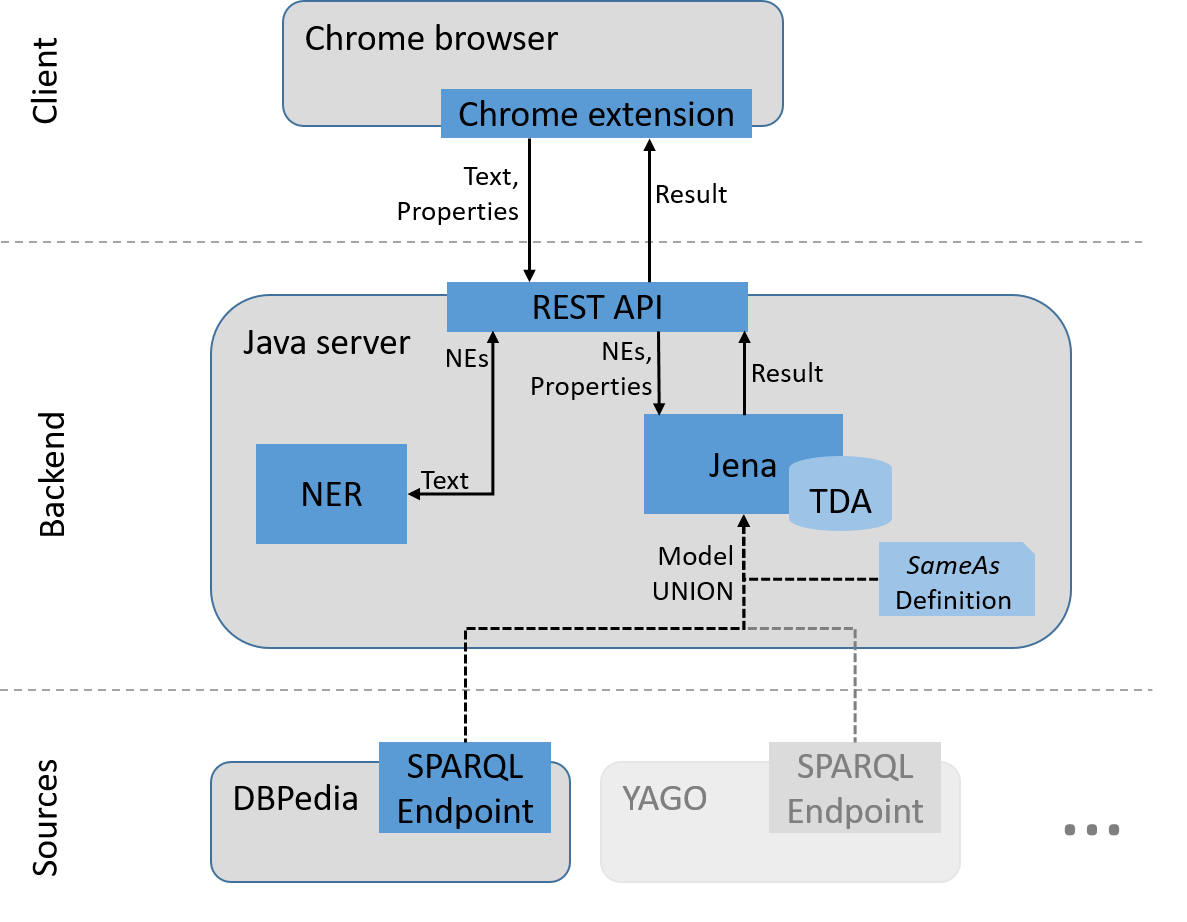
\includegraphics[width=0.6\textwidth]{architecture}
	\caption{High-Level Architecture}
	\label{fig:architecture}
\end{figure}



\subsection{Named Entity Recognition}
%Olli
%TODO: Describe NER via Stanford Core NLP

\subsection{SPARQL Queries}
After identifying the named entity and its entity type these information are handed over to the query engine which is implemented using Jena\footnote{\url{https://jena.apache.org/}}. The query process is divided into two steps, first all selected sources are queried in parallel in own threads and afterwards after all are finished the results are merged into one model where the result properties and the context triples are derived from. These two steps are illustrated in Figure \ref{fig:details_query} and explained in more detail in the following.
\begin{figure}[ht]
	\centering
	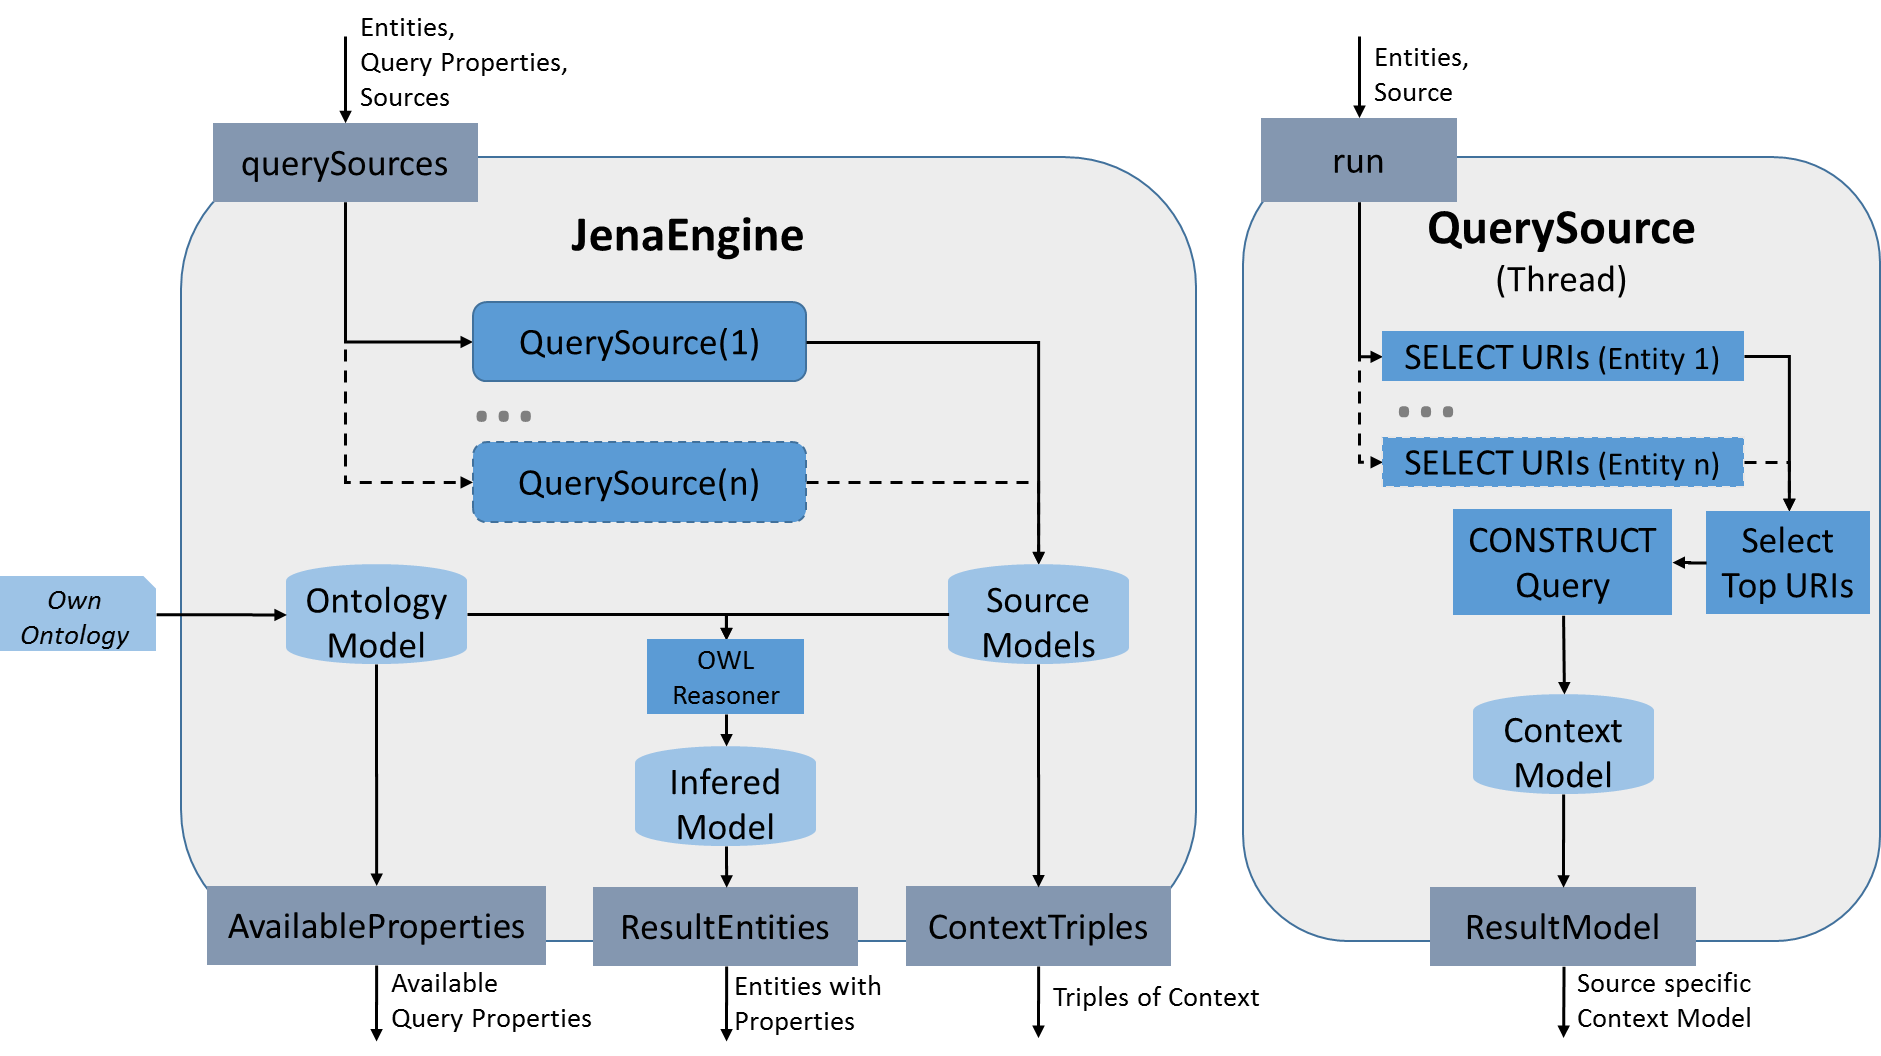
\includegraphics[width=1\textwidth]{QueryEngineDetails}
	\caption{Details of Query Engine}
	\label{fig:details_query}
\end{figure}

\paragraph{Querying Sources}
All sources are queried the same way via class QuerySource as illustrated in Figure \ref{fig:details_query} on the right hand side. Source queries could be generalized since the only differences are the endpoint URLs and entity type URIs as described before. In order to derive properties and context of a source based on the names and types of the entities, multiple queries are executed in two steps.

First step is the identification of URI candidates by performing a reg-ex based search per identified entity in the context. These queries run in parallel so the system can handle multiple entities without significant increase in runtime. Technically multiple \textit{SELECT-Queries} are executed, as shown in Figure \ref{fig:details_query}. The results of these first queries are URIs which meet the type definition and the reg-ex. The reg-ex allows up to 10 characters before and after the identified name and a period is replaces with ".*" to allow a match with shortened names. In cases there are too many matches (currently the threshold is five), an extended logic is used to reduce the amount of URI candidates. 

The approach for URI selection is based on a score which is calculated for each URI by multiplying a \textit{relation score} and the normalized edit distance of the URI label and the entity name. Therefore the source queries provide a count of relations available per URI. This information is used to calculate the \textit{relation score}, which is a relative score, being 1 for the URI with the most relations. The top five URIs with the highest score are selected. Less URIs are selected if there are not enough URIs having at least a score value of at least 75\% of the highest score value.

In a second step the identified URI candidates are used to query the source specific context. So all properties are queried as well as direct and in-direct relations between the entities. Furthermore the labels of all elements are derived as well as OWL \textit{sameAs} relations. 
This last query is a \textit{Construct-Query} and therefore returns a model which is the result of the source queries, as shown in Figure \ref{fig:details_query}. 

\paragraph{Querying Local Model}
After all source queries are finished the derived models are added to the same local model, as illustrated in Figure \ref{fig:details_query} on the left hand side. This model is combined with an own ontology defined for this project. This own ontology mainly consists of OWL \textit{euivelantProperty} definitions for own properties which group the corresponding sources specific properties. Furthermore there is a mapping of own classes representing the entity types to the corresponding source specific class definitions of the entities. Therefore the OWL \textit{equivelantClass} property is used. For inference the \textit{OWLMicroReasoner} is used. More complex OWL reasoner need much more time, so they are not used for performance reasons. 

Before the properties are derived from this inferred model, one URI per entity is derived across sources. The one with most relations is chosen. 
For these URIs the properties are then queried based on the own ontology and returned as result. If there are multiple result values for a property all values are returned. If the same value occurs multiple times for the same property, a count is increased. For numeric values additional logic is applied to ensure proper formatting and unit references. All property values including a language tag which is not empty nor English are discarded.


\subsection{Server and Chrome Extension}
%TODO: Olli



\section{Example results}
What outcomes does the application provide? – How is are some user queries answered? 
%@Olli?

\section{Known limitations}
In which domains does the application not work? 
Are there queries which cannot be answered? – Why? 

How could you overcome those limitations, given more time?

We could mention papers describing techniques which could improve certain areas like LINDA \cite{boehm_linda:_2012} for entity matching. 


\section{Lessons learned}
%Sascha
Which challenges did you face?
- Named Entity Identification as URI
- Performance
- Rejected queries
- no sameAs definitions between data sets


What were the biggest obstacles?
- finding active and stable public SPARQL endpoints


What would you do differently next time?
- using local sources
%References
%Add own references in .bib file
\pagebreak
\bibliographystyle{apalike}
\bibliography{SWTReport_Sascha}  
%\bibliography{SWTReport_Sascha,SWTReport_Olli}


\end{document}
